% !TeX program = xelatex
% !TeX root = ./main.tex
\documentclass[10pt,aspectratio=169,xcolor={dvipsnames}]{beamer}

\usetheme{blei}
\AtBeginSection[]{}

\usepackage{xeCJK}
\usepackage{amsmath}
\usepackage{graphicx}
\usepackage{booktabs}
\usepackage{tikz}
\usetikzlibrary{arrows.meta,positioning,fit,calc}

\setCJKmainfont[AutoFakeBold=2,AutoFakeSlant=.2]{STSong}
\setCJKsansfont[AutoFakeBold=2,AutoFakeSlant=.2]{STSong}
\setCJKmonofont{STSong}
\setbeamertemplate{caption}{\raggedright\insertcaption\par}
\setbeamertemplate{caption label separator}{}
\setbeamersize{text margin left=1.3em,text margin right=1.3em}

\definecolor{rqblue}{RGB}{37,99,235}
\definecolor{rqred}{RGB}{185,28,28}
\definecolor{rqgreen}{RGB}{5,150,105}
\definecolor{rqgray}{RGB}{75,85,99}

\newcommand{\img}[2][]{\includegraphics[#1]{\detokenize{#2}}}
\newcommand{\keypoint}[1]{\textbf{#1}}
\newcommand{\method}[1]{\texttt{\small #1}}

\tikzset{
  box/.style={draw, rounded corners=1pt, align=center, minimum height=6mm, font=\scriptsize},
  quant/.style={draw=rqblue, fill=rqblue!6, text=rqblue, rounded corners=1pt, align=center, minimum height=7mm, font=\scriptsize},
  fp/.style={draw=rqred!70!black, fill=rqred!4, text=rqred!80!black, rounded corners=1pt, align=center, minimum height=6mm, font=\scriptsize},
  soft/.style={draw=rqgreen!70!black, fill=rqgreen!5, rounded corners=1pt, align=center, minimum height=6mm, font=\scriptsize},
  module/.style={draw=gray!65, dashed, rounded corners=2pt, inner sep=4pt},
  arrow/.style={-{Latex[length=1.8mm]}, thick},
  prep/.style={-{Latex[length=1.8mm]}, dashed, gray!70, thick},
  residual/.style={-{Latex[length=1.8mm]}, rqred, thick}
}

\title{Rotation-domain Fake Quantization}
\author{}
\date{}

\begin{document}

\begin{frame}{Hadamard Rotation 与 Lloyd-Max Quantization}
  \begin{columns}[T,onlytextwidth]
    \begin{column}{0.48\textwidth}
      \keypoint{计算不变性}
      \[
        H^{T}H=I,\qquad
        y=xW^{T}=(xH)(WH)^{T}
      \]
      \[
        QK^{T}=(QH)(KH)^{T}
      \]
      \vspace{-0.2em}
      \begin{itemize}
        \item Hadamard rotation 是正交换基；不量化时不改变 Linear / Attention score。
        \item Rotation 负责平滑 outlier，使 block / head 内 scale 更稳定。
        \item Rotation 后激活值分布更趋于 Gaussian 分布，是适配 Lloyd-Max 量化的先决条件。
      \end{itemize}
    \end{column}
    \begin{column}{0.48\textwidth}
      \keypoint{Lloyd-Max codebook}
      \[
        \hat{x}=s\cdot c_{i^{*}},\qquad
        i^{*}=\arg\min_i \left|x/s-c_i\right|
      \]
      \vspace{-0.4em}
      \begin{center}
      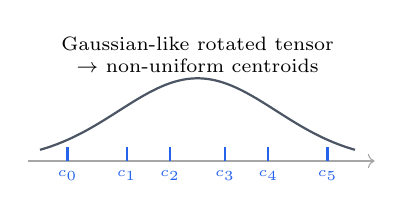
\begin{tikzpicture}[x=1cm,y=1cm]
        \draw[->, gray!70] (-2.15,0) -- (2.25,0);
        \draw[domain=-2:2,samples=80,thick,rqgray] plot (\x,{1.05*exp(-0.5*\x*\x)});
        \foreach \x/\lab in {-1.65/$c_0$,-0.9/$c_1$,-0.35/$c_2$,0.35/$c_3$,0.9/$c_4$,1.65/$c_5$} {
          \draw[rqblue, thick] (\x,0) -- (\x,0.18);
          \node[font=\tiny, text=rqblue] at (\x,-0.18) {\lab};
        }
        \node[font=\scriptsize, align=center] at (0,1.35) {Gaussian-like rotated tensor\\$\rightarrow$ non-uniform centroids};
      \end{tikzpicture}
      \end{center}
      \begin{itemize}
        \item Lloyd-Max 在 RMS 标准化后的近似 Gaussian 分布上最小化 MSE。
        \item Lloyd-Max 量化结果是 fixed centroid codebook，通过索引 dequant。
        \item 后续硬件协同设计可考虑 LUT-based 计算单元。
      \end{itemize}
    \end{column}
  \end{columns}
\end{frame}

\begin{frame}{当前模型量化计算流}
  \vspace{-0.3em}
  \begin{center}
  \resizebox{0.98\linewidth}{!}{%
  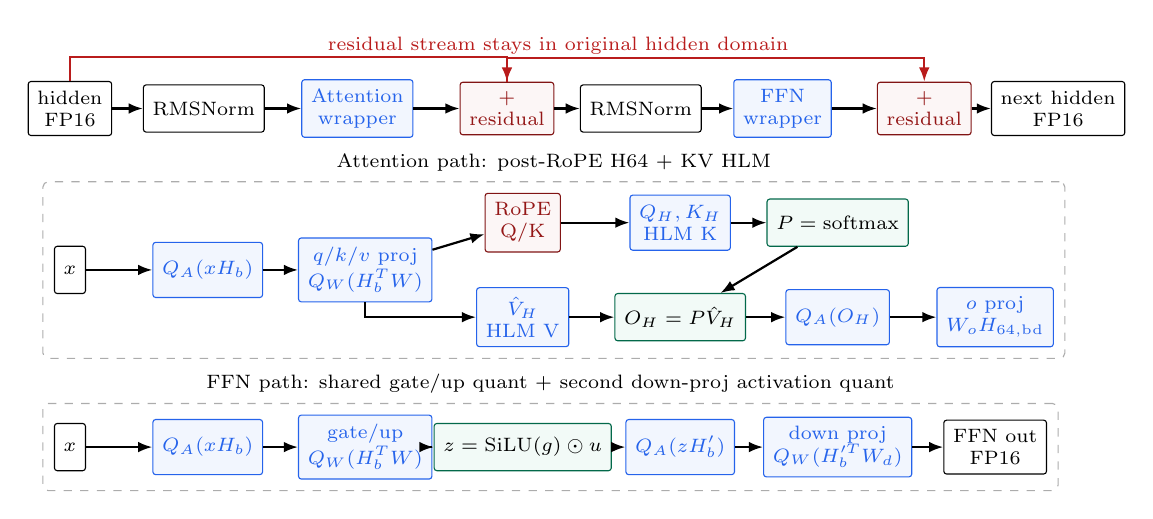
\begin{tikzpicture}[x=1cm,y=1cm]
    \node[box] (h0) at (0,0.30) {hidden\\FP16};
    \node[box] (rn1) at (1.7,0.30) {RMSNorm};
    \node[quant] (attn) at (3.65,0.30) {Attention\\wrapper};
    \node[fp] (add1) at (5.55,0.30) {$+$\\residual};
    \node[box] (rn2) at (7.25,0.30) {RMSNorm};
    \node[quant] (ffn) at (9.05,0.30) {FFN\\wrapper};
    \node[fp] (add2) at (10.85,0.30) {$+$\\residual};
    \node[box] (h1) at (12.55,0.30) {next hidden\\FP16};
    \draw[arrow] (h0) -- (rn1);
    \draw[arrow] (rn1) -- (attn);
    \draw[arrow] (attn) -- (add1);
    \draw[arrow] (add1) -- (rn2);
    \draw[arrow] (rn2) -- (ffn);
    \draw[arrow] (ffn) -- (add2);
    \draw[arrow] (add2) -- (h1);
    \draw[residual] (h0.north) -- ++(0,0.30) -| (add1.north);
    \draw[residual] (add1.north) -- ++(0,0.30) -| (add2.north);
    \node[font=\scriptsize, text=rqred] at (6.2,1.10) {residual stream stays in original hidden domain};

    \node[box] (ax) at (0,-1.75) {$x$};
    \node[quant] (aq) at (1.75,-1.75) {$Q_A(xH_b)$};
    \node[quant] (qkv) at (3.75,-1.75) {$q/k/v$ proj\\$Q_W(H_b^TW)$};
    \node[fp] (rope) at (5.75,-1.15) {RoPE\\Q/K};
    \node[quant] (qk) at (7.75,-1.15) {$Q_H,K_H$\\HLM K};
    \node[soft] (score) at (9.75,-1.15) {$P=\mathrm{softmax}$};
    \node[quant] (vh) at (5.75,-2.35) {$\hat{V}_H$\\HLM V};
    \node[soft] (oh) at (7.75,-2.35) {$O_H=P\hat{V}_H$};
    \node[quant] (oq) at (9.75,-2.35) {$Q_A(O_H)$};
    \node[quant] (op) at (11.75,-2.35) {$o$ proj\\$W_oH_{64,\mathrm{bd}}$};
    \draw[arrow] (ax) -- (aq);
    \draw[arrow] (aq) -- (qkv);
    \draw[arrow] (qkv) -- (rope);
    \draw[arrow] (rope) -- (qk);
    \draw[arrow] (qk) -- (score);
    \draw[arrow] (qkv) |- (vh);
    \draw[arrow] (score) -- (oh);
    \draw[arrow] (vh) -- (oh);
    \draw[arrow] (oh) -- (oq);
    \draw[arrow] (oq) -- (op);
    \node[module, fit=(ax)(op)(rope)(vh), label={[font=\scriptsize]above:Attention path: post-RoPE H64 + KV HLM}] {};

    \node[box] (fx) at (0,-4.0) {$x$};
    \node[quant] (fq) at (1.75,-4.0) {$Q_A(xH_b)$};
    \node[quant] (gu) at (3.75,-4.0) {gate/up\\$Q_W(H_b^TW)$};
    \node[soft] (silu) at (5.75,-4.0) {$z=\mathrm{SiLU}(g)\odot u$};
    \node[quant] (fq2) at (7.75,-4.0) {$Q_A(zH'_b)$};
    \node[quant] (down) at (9.75,-4.0) {down proj\\$Q_W(H_b'^TW_d)$};
    \node[box] (fy) at (11.75,-4.0) {FFN out\\FP16};
    \draw[arrow] (fx) -- (fq);
    \draw[arrow] (fq) -- (gu);
    \draw[arrow] (gu) -- (silu);
    \draw[arrow] (silu) -- (fq2);
    \draw[arrow] (fq2) -- (down);
    \draw[arrow] (down) -- (fy);
    \node[module, fit=(fx)(fy)(gu)(fq2), label={[font=\scriptsize]above:FFN path: shared gate/up quant + second down-proj activation quant}] {};
  \end{tikzpicture}}
  \end{center}
  \vspace{-0.2em}
  {\footnotesize 主要关注：\method{Rot-LM W4A4 + HLM K4V4}；Attention 与 FFN 分别替换 \method{self\_attn} 和 \method{mlp}，$Q_A(\cdot)$ 和 $Q_W(\cdot)$ 分别表示 activation / weight quantizer。}
\end{frame}

\begin{frame}{Full-model PPL实验结果}
  \begin{columns}[T,onlytextwidth]
    \begin{column}{0.67\textwidth}
      \vspace{-0.4em}
      \img[width=\linewidth,height=0.55\textheight,keepaspectratio]{image/full_model_ppl.pdf}
    \end{column}
    \begin{column}{0.31\textwidth}
      \footnotesize
      \begin{itemize}
        \setlength{\itemsep}{0.35em}
        \item \keypoint{Best 4-bit:}\\
        Full Rot-LM W4A4 + HLM K4V4，PPL = \textbf{9.23}.
        \item \keypoint{Baselines:}\\
        MXFP4 = 10.26，Direct Absmax = 11.12，Rot-MXFP4 = 10.15.
        \item \keypoint{Rotation backend:}\\
        Hadamard / Rand-Hadamard / Rand-Ortho 分别为 9.23 / 9.37 / 9.80。
        \item \keypoint{Block size:}\\
        W4A4 下 32/64/128 接近，block size取64结果最优。
      \end{itemize}
    \end{column}
  \end{columns}
\end{frame}

\begin{frame}{后续方向：FWHT + LUT-based Codebook Compute}
  \begin{columns}[T,onlytextwidth]
    \begin{column}{0.48\textwidth}
      \keypoint{Rotation path: FWHT butterfly}
      \vspace{0.25em}
      \begin{center}
        \img[width=\linewidth,height=0.36\textheight,keepaspectratio]{../figures/FWHT.png}
      \end{center}
      \footnotesize
      \begin{itemize}
        \setlength{\itemsep}{0.35em}
        \item Hadamard rotation 可由 FWHT 实现，核心为 add/sub 与 routing。
        \item 支持 H32 / H64 / H128 block-local rotation，避免 dense matrix multiply。
      \end{itemize}
    \end{column}
    \begin{column}{0.48\textwidth}
      \keypoint{Linear path: LUT-based Lloyd-Max MAC}
      \vspace{0.25em}
      \begin{center}
      \resizebox{\linewidth}{!}{%
      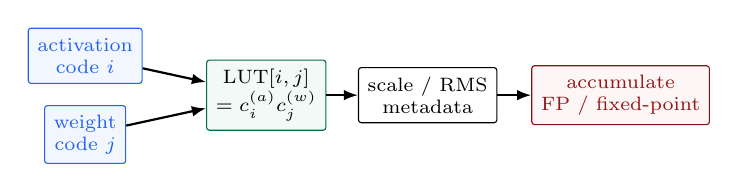
\begin{tikzpicture}[x=1cm,y=1cm]
        \node[quant] (acode) at (0,0) {activation\\code $i$};
        \node[quant] (wcode) at (0,-1.0) {weight\\code $j$};
        \node[soft] (lut) at (2.3,-0.5) {$\mathrm{LUT}[i,j]$\\$=c_i^{(a)}c_j^{(w)}$};
        \node[box] (scale) at (4.35,-0.5) {scale / RMS\\metadata};
        \node[fp] (acc) at (6.8,-0.5) {accumulate\\FP / fixed-point};
        \draw[arrow] (acode) -- (lut);
        \draw[arrow] (wcode) -- (lut);
        \draw[arrow] (lut) -- (scale);
        \draw[arrow] (scale) -- (acc);
      \end{tikzpicture}}
      \end{center}
      \footnotesize
      \begin{itemize}
        \setlength{\itemsep}{0.35em}
        \item Lloyd-Max 存储 codebook index，计算需要 centroid lookup。
        \item 设计Codebook-aware RQ-GEMM kernel 或 Fused FWHT + RQ-GEMM kernel。
        \item 对比：GPU上的 INT4 GEMM kernel 和 FPGA上实现的 Naive dequantize-then-MAC FPGA kernel。
      \end{itemize}
    \end{column}
  \end{columns}
\end{frame}

\end{document}
